% based on an example in the tikzpeople manual
\documentclass[tikz,border=2pt]{standalone}
\usepackage{tikzpeople}
\begin{document}
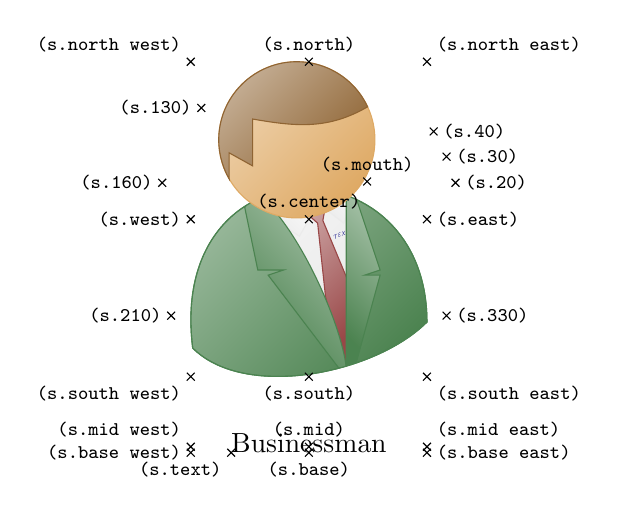
\begin{tikzpicture}
  \node[name=s, shape=businessman, monogramtext=TEX, minimum width=3cm]
    {Businessman\rule{0pt}{0.8cm}};
  \foreach \anchor/\placement in
    { north west/above left, north/above, north east/above right,
      west/left, center/above, east/right,				
      mid west/above left, mid/above, mid east/above right,
      base west/left, base/below, base east/right,
      south west/below left, south/below, south east/below right,
      text/below left, 20/right, 30/right, 40/right, 130/left, 
	  160/left, 210/left, 330/right, mouth/above}
  \draw[shift=(s.\anchor)] plot[mark=x] coordinates{(0,0)}
    node[\placement] {\scriptsize\texttt{(s.\anchor)}};
\end{tikzpicture}
\end{document}
